\documentclass[20pt]{report}
\usepackage[a4paper]{geometry}
\usepackage[myheadings]{fullpage}
\usepackage{fancyhdr}
\usepackage{lastpage}
\usepackage{graphicx, wrapfig, subcaption, setspace, booktabs}
\usepackage[T1]{fontenc}
\usepackage[font=large, labelfont=bf]{caption}
\usepackage{fourier}
\usepackage[protrusion=true, expansion=true]{microtype}
\usepackage[english]{babel}
\usepackage{sectsty}
\usepackage{url}
\usepackage{amsmath}
\newcommand{\HRule}[1]{\rule{\linewidth}{#1}}
\onehalfspacing
\setcounter{tocdepth}{5}
\setcounter{secnumdepth}{5}
\pagestyle{fancy}
\fancyhf{}
\setlength\headheight{25pt}
%\fancyhead[L]{Group No: 12}
%\fancyhead[R]{Linear Algebra and Random Process}
%\fancyfoot[R]{Page \thepage\ of \pageref{LastPage}}


\begin{document}
\title{ \normalsize \textsc{CS7015 : Deep Learning}
		\\ [2.0cm]\HRule{0.5pt} \\
        \LARGE \textbf{\uppercase{Report of Programming Assignment-1}}
		\HRule{2pt} \\ [0.5cm]
		\normalsize \today \vspace*{5\baselineskip}}
\date{}
\author{Niraj Kumar Singh\\BS13B028\\Sweta Kumari\\BT17D019\\Indian Institute of Technology Madras\\Chennai-600036 }
\maketitle
%\tableofcontents
\newpage
\sectionfont{\scshape}
\textbf{Problem:-1, 2, 3, 4}\\
Red---> Validation Loss
Blue---> Training Loss
\\
\textbf{Number of Hidden Layer:-1}\\
\begin{figure}[!htb]
\minipage{0.2\textwidth}
  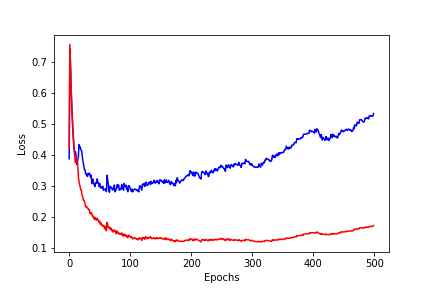
\includegraphics[width=\linewidth]{1_50.png}
	\caption{50}
\endminipage\hfill
\minipage{0.2\textwidth}
  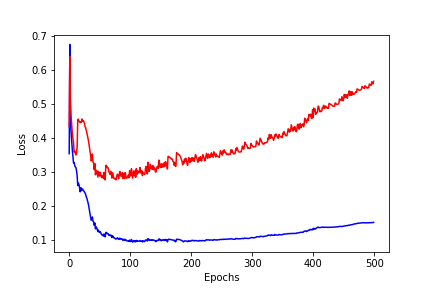
\includegraphics[width=\linewidth]{1_100.png}
	\caption{100}
\endminipage\hfill
\minipage{0.2\textwidth}
  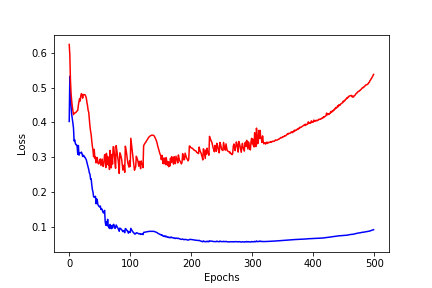
\includegraphics[width=\linewidth]{1_200.png}
	\caption{200}
\endminipage\hfill
\minipage{0.2\textwidth}
  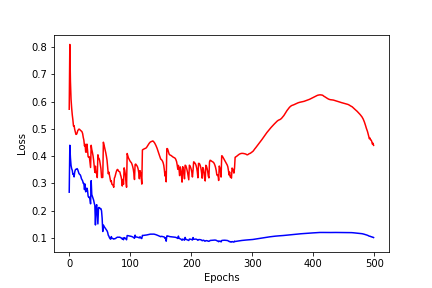
\includegraphics[width=\linewidth]{1_300.png}
	\caption{300}
\endminipage\hfill
\\\\
\textbf{Number of Hidden Layer:-2}\\\\
\minipage{0.2\textwidth}
  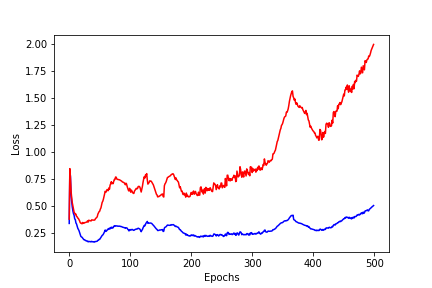
\includegraphics[width=\linewidth]{2_50.png}
	\caption{50}
\endminipage\hfill
\minipage{0.2\textwidth}
  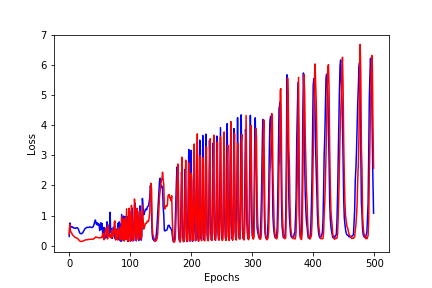
\includegraphics[width=\linewidth]{2_100.png}
	\caption{100}
\endminipage\hfill
\minipage{0.2\textwidth}
  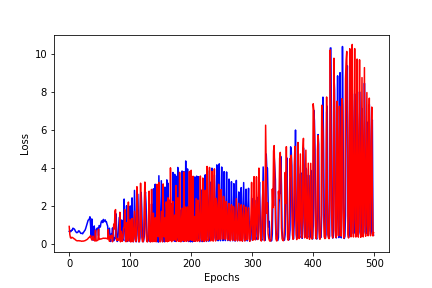
\includegraphics[width=\linewidth]{2_200.png}
	\caption{200}
\endminipage\hfill
\minipage{0.2\textwidth}
  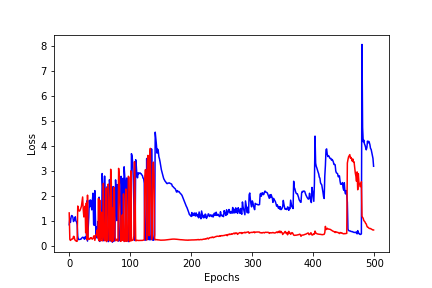
\includegraphics[width=\linewidth]{2_300.png}
	\caption{300}
\endminipage\hfill
\caption{Adam, BatchSize = 55000, LearningRate = 0.001, Epochs=5000.}
\end{figure}
\\\\
\textbf{Number of Hidden Layer:-3}\\
\begin{figure}[!htb]
\minipage{0.2\textwidth}
  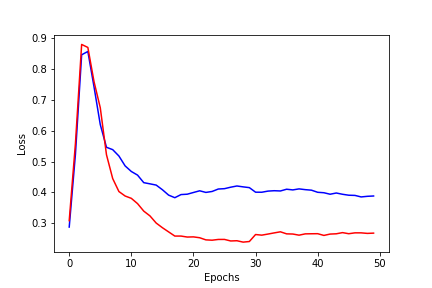
\includegraphics[width=\linewidth]{3_50.png}
	\caption{50}
\endminipage\hfill
\minipage{0.2\textwidth}
  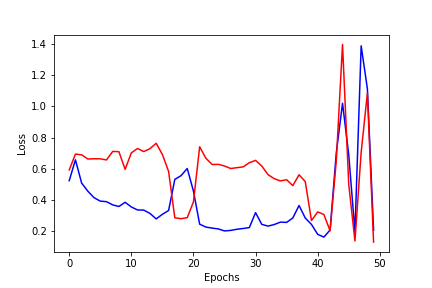
\includegraphics[width=\linewidth]{3_100.png}
	\caption{100}
\endminipage\hfill
\minipage{0.2\textwidth}
  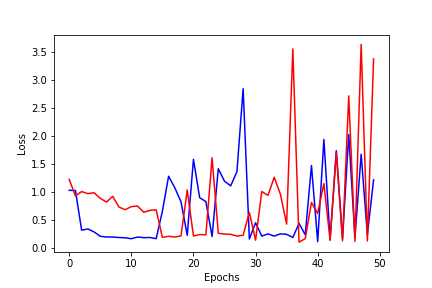
\includegraphics[width=\linewidth]{3_200.png}
	\caption{200}
\endminipage\hfill
\minipage{0.2\textwidth}
  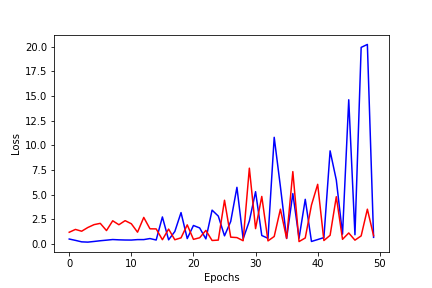
\includegraphics[width=\linewidth]{3_300.png}
	\caption{300}
\endminipage\hfill
\\\\
\textbf{Number of Hidden Layer:-4}\\\\
\minipage{0.2\textwidth}
  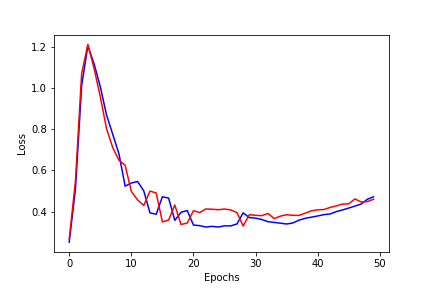
\includegraphics[width=\linewidth]{4_50.png}
	\caption{50}
\endminipage\hfill
\minipage{0.2\textwidth}
  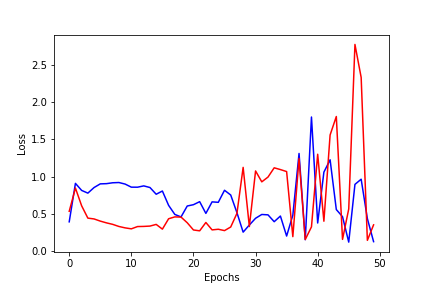
\includegraphics[width=\linewidth]{4_100.png}
	\caption{100}
\endminipage\hfill
\minipage{0.2\textwidth}
  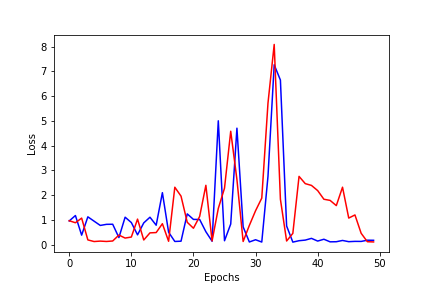
\includegraphics[width=\linewidth]{4_200.png}
	\caption{200}
\endminipage\hfill
\minipage{0.2\textwidth}
  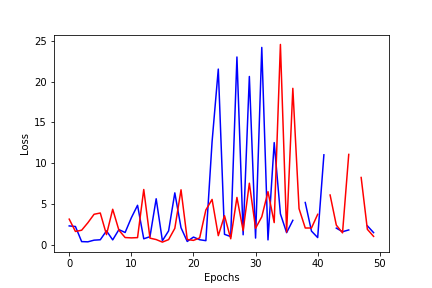
\includegraphics[width=\linewidth]{4_300.png}
	\caption{300}
\endminipage\hfill
 \caption{Adam, BatchSize = 55000, LearningRate = 0.001, Epochs=500.}
\end{figure}


%\\\\
%\textbf{Problem:- 5}\\
%\\
%\textbf{Number of Hidden Layer:-3 and Number of Neurons:- 300}\\
%\begin{figure}[!htb]
%\minipage{0.2\textwidth}
%  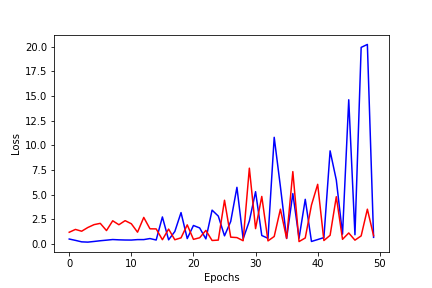
\includegraphics[width=\linewidth]{3_300.png}
%	\caption{Adam}
%\endminipage\hfill
%\minipage{0.2\textwidth}
%  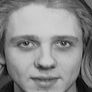
\includegraphics[width=\linewidth]{fce1.jpg}
%	\caption{NAG}
%\endminipage\hfill
%\minipage{0.2\textwidth}
%  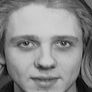
\includegraphics[width=\linewidth]{fce1.jpg}
%	\caption{Momentum}
%\endminipage\hfill
%\minipage{0.2\textwidth}
%  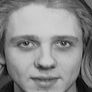
\includegraphics[width=\linewidth]{fce1.jpg}
%	\caption{GD}
%\endminipage\hfill
%\caption{MiniBatch = 55000, LearningRate = 0.001, Epochs=5000.}
%\end{figure}
%\\
%\textbf{Problem:- 6}\\
%\\
%\textbf{Number of Hidden Layer:-2 and Number of Neurons:- 100}\\
%\begin{figure}[!htb]
%\minipage{0.4\textwidth}
%  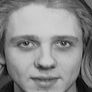
\includegraphics[width=\linewidth]{fce1.jpg}
%	\caption{Sigmoid}
%\endminipage\hfill
%\minipage{0.4\textwidth}
%  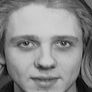
\includegraphics[width=\linewidth]{fce1.jpg}
%	\caption{Tanh}
%	\endminipage\hfill
%\caption{Adam, MiniBatch = 55000, LearningRate = 0.001, Epochs=5000.}
%\end{figure}
%\\
%\textbf{Problem:- 7}\\
%\\
%\textbf{Number of Hidden Layer:-2 and Number of Neurons:- 100}\\
%\begin{figure}[!htb]
%\minipage{0.4\textwidth}
%  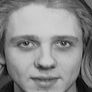
\includegraphics[width=\linewidth]{fce1.jpg}
%	\caption{Cross Entropy Loss}
%\endminipage\hfill
%\minipage{0.4\textwidth}
%  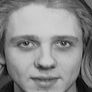
\includegraphics[width=\linewidth]{fce1.jpg}
%	\caption{Squared Error Loss}
%	\endminipage\hfill
%\caption{Adam, MiniBatch = 55000, LearningRate = 0.001, Epochs=5000.}
%\end{figure}
%\\\\\\\\
%\textbf{Problem:- 8}
%\\
%\textbf{Number of Hidden Layer:-2 and Number of Neurons:- 100}\\
%\begin{figure}[!htb]
%\minipage{0.2\textwidth}
%  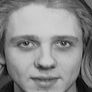
\includegraphics[width=\linewidth]{fce1.jpg}
%	\caption{Batch Size = 1}
%\endminipage\hfill
%\minipage{0.2\textwidth}
%  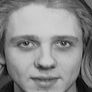
\includegraphics[width=\linewidth]{fce1.jpg}
%	\caption{Batch Size = 20}
%\endminipage\hfill
%\minipage{0.2\textwidth}
%  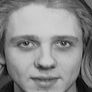
\includegraphics[width=\linewidth]{fce1.jpg}
%	\caption{Batch Size = 100}
%\endminipage\hfill
%\minipage{0.2\textwidth}
%  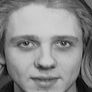
\includegraphics[width=\linewidth]{fce1.jpg}
%	\caption{Batch Size = 1000}
%\endminipage\hfill
%\caption{MiniBatch = 55000, LearningRate = 0.001, Epochs=5000.}
%\end{figure}





\end{document}